%!TEX TS-program = xelatex
%!TEX encoding = UTF-8 Unicode
%% Author : Haoran You
%% Date   : 1.1.2018

\documentclass[UTF-8,a4paper, 12pt]{article}

%%%%%% 导入包 %%%%%%
\usepackage{xeCJK}
\usepackage{graphicx}
\usepackage[unicode]{hyperref}
\hypersetup{colorlinks=true,linkcolor=black}
\usepackage{xcolor}
\usepackage{cite}
\usepackage{indentfirst}
\usepackage{amsmath}
\numberwithin{equation}{section}
\usepackage{amssymb}
\usepackage{chemfig}
\usepackage{cite}
\usepackage{times}

\usepackage{ctex}
\usepackage{geometry}
\usepackage{graphicx}
\usepackage{multirow}
\usepackage{array}
\usepackage{titlesec}
\usepackage{float}

% \usepackage[colorlinks,linkcolor=red]{hyperref}
\usepackage[super,square,comma,sort&compress]{natbib}
\usepackage{listings}
\usepackage{xcolor}

\colorlet{punct}{red!60!black}
\definecolor{background}{HTML}{EEEEEE}
\definecolor{delim}{RGB}{20,105,176}
\colorlet{numb}{magenta!60!black}

\lstdefinelanguage{json}{
    basicstyle=\ttfamily\scriptsize,
    numbers=left,
    numberstyle=\ttfamily\scriptsize,
    stepnumber=1,
    numbersep=4pt,
    showstringspaces=false,
    breaklines=true,
    frame=lines,
    % backgroundcolor=\color{background},
    literate=
     *{0}{{{\color{numb}0}}}{1}
      {1}{{{\color{numb}1}}}{1}
      {2}{{{\color{numb}2}}}{1}
      {3}{{{\color{numb}3}}}{1}
      {4}{{{\color{numb}4}}}{1}
      {5}{{{\color{numb}5}}}{1}
      {6}{{{\color{numb}6}}}{1}
      {7}{{{\color{numb}7}}}{1}
      {8}{{{\color{numb}8}}}{1}
      {9}{{{\color{numb}9}}}{1}
      {:}{{{\color{punct}{:}}}}{1}
      {,}{{{\color{punct}{,}}}}{1}
      {\{}{{{\color{delim}{\{}}}}{1}
      {\}}{{{\color{delim}{\}}}}}{1}
      {[}{{{\color{delim}{[}}}}{1}
      {]}{{{\color{delim}{]}}}}{1},
}


\lstset{
    columns=flexible,
    tabsize = 4,
    basicstyle=\ttfamily\scriptsize,                     % 字体大小
    backgroundcolor=\color{white},                       % 背景颜色
    numbers=left,                                        % 在左侧显示行号
    keywordstyle=\color[RGB]{40,40,255},                 % 设定关键字颜色
    % frame=trbl,
    stepnumber=1,
    numbersep=4pt,
    breaklines=true,
    frame=lines,
    numberstyle=\ttfamily\scriptsize\color{darkgray},    % 设定行号格式
    commentstyle=\it\color[RGB]{0,96,96},                % 设置代码注释的格式
    stringstyle=\rmfamily\slshape\color[RGB]{128,0,0},   % 设置字符串格式
    showstringspaces=false,                              % 不显示字符串中的空格
    language=python,                                     % 设置语言
}

\graphicspath{{figure/}}

\usepackage{geometry}
\geometry{a4paper,left=2.5cm,right=2.5cm,top=2cm,bottom=3cm}

%%%%%% 设置字号 %%%%%%
\newcommand{\chuhao}{\fontsize{42pt}{\baselineskip}\selectfont}
\newcommand{\xiaochuhao}{\fontsize{36pt}{\baselineskip}\selectfont}
\newcommand{\yihao}{\fontsize{28pt}{\baselineskip}\selectfont}
\newcommand{\erhao}{\fontsize{21pt}{\baselineskip}\selectfont}
\newcommand{\xiaoerhao}{\fontsize{18pt}{\baselineskip}\selectfont}
\newcommand{\sanhao}{\fontsize{15.75pt}{\baselineskip}\selectfont}
\newcommand{\sihao}{\fontsize{14pt}{\baselineskip}\selectfont}
\newcommand{\xiaosihao}{\fontsize{12pt}{\baselineskip}\selectfont}
\newcommand{\wuhao}{\fontsize{10.5pt}{\baselineskip}\selectfont}
\newcommand{\xiaowuhao}{\fontsize{9pt}{\baselineskip}\selectfont}
\newcommand{\liuhao}{\fontsize{7.875pt}{\baselineskip}\selectfont}
\newcommand{\qihao}{\fontsize{5.25pt}{\baselineskip}\selectfont}


%%%% 设置 font 属性 %%%%
%设置中文正体字体,BoldFont设置粗体和斜体样式对应的字体
\setCJKmainfont[BoldFont ={STXihei},ItalicFont ={STKaiti}]{STSong}
\setCJKsansfont{STXihei}    %设置无衬线样式对应字体
\setCJKmonofont{STSong}     %设置有衬线样式对应字体
\punctstyle{hangmobanjiao}  %行末半角式:所有标点占一个汉字宽度,行首行末对齐

%%%% 设置 section 属性 %%%%
\titlespacing*{\section} {9pt}{-0.5ex plus .1ex minus .2ex}{-0.8ex plus -.1ex}
\titlespacing*{\subsection} {8pt}{-.8ex plus .1ex minus .2ex}{-1.1ex plus -.1ex}
\titlespacing*{\subsubsection}{8pt}{-.1ex plus .1ex minus .2ex}{-1.1ex plus -.1ex}

\titleformat*{\section}{\Large\bfseries\sffamily\color{black}} % \color{blue}
\titleformat*{\subsection}{\large\bfseries\sffamily\color{black}}
\titleformat*{\subsubsection}{\normalsize\bfseries\sffamily\color{black}} % \subsubsectionfont}

%%%% 段落首行缩进两个字 %%%%
\makeatletter
\let\@afterindentfalse\@afterindenttrue
\@afterindenttrue
\makeatother
\setlength{\parindent}{2em}  %中文缩进两个汉字位

\linespread{1.2}
% \setlength{\parskip}{1ex}
\setlength{\parskip}{0.6\baselineskip}

\renewcommand{\thetable}{\thesection.\arabic{table}}
\renewcommand{\thefigure}{\thesection.\arabic{figure}}

%%%% 正文开始 %%%%
\begin{document}

\begin{titlepage}
    \begin{center}
    \phantom{Start!}
	\vspace{2cm}
	
\includegraphics[width=350pt]{HuaKe.jpg} \\
     \center{
          \vspace{0.5cm}
          \textbf{\xiaochuhao 电子信息与通信学院}\\
       	  \vspace{1cm}
       	  \textbf{\yihao 实\quad 验\quad 报\quad 告}\\
       	  \vspace{0.5cm}
          \textbf{\sanhao (2017 / 2018学年\quad 第1学期)}
      }
      \vspace{2cm}
      \begin{table}[!hbp]
      \centering
      \renewcommand\arraystretch{1.5}
     	\begin{tabular}{|c|c|}
     		\hline
     		课程名称 & 软件课设\\
     		\hline
     		实验名称 & ~~~~~~面向知乎QAWEB的网络爬虫设计与实现 ~~~~~~ \\
     		\hline
            指导教师 & 魏蛟龙 \\
     		\hline
            课程助教& 聂锦燃  \\
            \hline
            小组成员& 游浩然 \quad 黎张帆 \quad 郭金城 \\
            \hline
     		\end{tabular}     		
       \end{table}
       \vspace{2.5cm}
      \begin{table}[!htbp]
      \centering
      \renewcommand\arraystretch{1.5}
     	\begin{tabular}{|c|c|c|c|}
     		\hline
            \qquad ~~姓名~~~~~  & \qquad ~~游浩然~~~~~  & \qquad 学号~~~~~ & \qquad U201515429~~~~~ \\
            \hline
     		\end{tabular}
       \end{table}
     \end{center}
     \vspace{1cm}
     \centerline{\large{\today}}
\end{titlepage}

\tableofcontents
\newpage

\section{设计目的}
\vspace {0.2cm}
\begin{itemize}
  \item 加深对网络框架、协议及软件编程技术的理解
  \item 锻炼网络编程与解决实际问题的能力
  \item 熟练利用Python进行算法实现,培养将专业技能转换为实践的能力
\end{itemize}

\section{开发平台}
\begin{itemize}
  \item 硬件平台:个人PC,可连接WEB网络
  \item 软件环境:
  \begin{itemize}
    \item 操作系统:WINDOWS 10 \& Ubuntu
    \item IDE:PyCharm Community Edition 2017.2.3
    \item Python版本:Python 3.6.3 |Anaconda, Inc.| (default, Oct 15 2017, 03:27:45)
  \end{itemize}
  \item 项目所需库
  \begin{itemize}
    \item Wxpthon: Python GUI库
    \item Selenium: Python 模拟浏览器操作库
    \item Phantom:基于selenium的Python工业化模拟浏览器操作库,需设置运行路径或将bin文件夹放入系统路径中。
  \end{itemize}
\end{itemize}
\section{项目描述}
随着时代发展,网络成为大量信息的载体,如何有效地提取并利用这些信息成为一个巨大的挑战,定向抓取相关网页资源的“爬虫”也应运而生。爬虫不追求大的覆盖,而将目标定为抓取与某一特定主题内容相关的网页,为面向主题的用户查询准备数据资源。
传统爬虫从一个初始网页的URL开始,获得初始网页上的URL,在抓取网页的过程中,不断从当前页面抓取新的URL放入队列,直到满足系统的一定停止条件。爬虫程序主要有三个模块:
\begin{itemize}
  \item 爬虫控制端:启动爬虫,停止爬虫,监视爬虫的运行情况
  \item 爬虫运行模块:包含三个小模块,URL管理器、网页下载器、网页解析器
  \begin{itemize}
    \item URL管理器:对需要爬取的URL和已经爬取过的URL进行管理,可以从其中取出待爬取的URL传递给网页下载器。
    \item 网页下载器:网页下载器将URL指定的网页下载下来,存储成一个字符串,传递给网页解析器。
    \item 网页解析器:网页解析器解析传递的字符串,解析器不仅可以解析出需要爬取的数据,而且还可以解析出每一个网页指向其他网页的URL,这些URL被解析出来会补充进URL管理器。
  \end{itemize}
  \item 数据输出模块:存储爬取的数据
\end{itemize}

本课程实验借鉴其方法,对知乎中特定的问题(question)或者话题(topic)进行定向爬取。从知乎首页(\url{http://www.zhihu.com})开始进入,输入关键词,以广度优先的方式,爬取相关联的网页显示的相关信息,包括问题本体、问题的提出者、浏览次数、点赞/差评次数、答案、答案的作者、答案的评论、答案获得的点赞/差评数,最后以json格式存取。

\section{软件设计}
\subsection{整体框架设计}
通过主程序调用知乎登陆函数,显示GUI界面,根据GUI界面所获取的搜索任务信息来爬取URL,补充问题URL池,等待问题的URL爬取完毕,开始对每一个问题的URL爬取相应内容。\\
各模块之间的关系如下图所示:
\begin{figure}[!htbp]
  \centering
  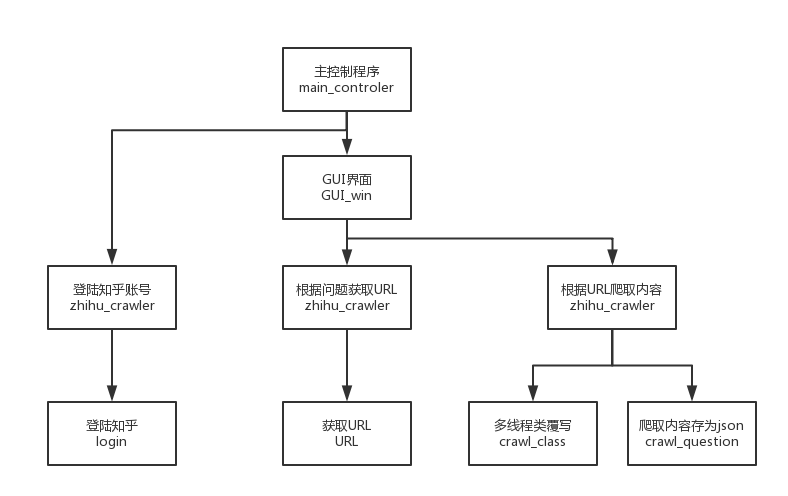
\includegraphics[width=15cm,height=9cm]{模块关系}
  \caption{各模块之间调用关系}\label{模块关系}
\end{figure}

程序运行的逻辑关系如下图所示:
\begin{figure}[!htbp]
  \centering
  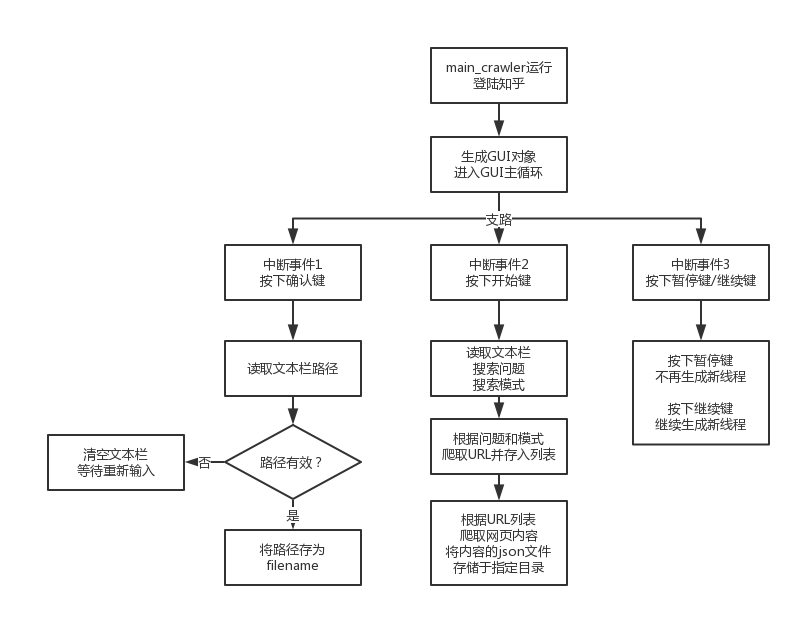
\includegraphics[width=15cm,height=11cm]{主程序流程图}
  \caption{程序逻辑关系}\label{主程序流程图}
\end{figure}
\newpage
% 程序代码详见:\url{https://github.com/ranery/ZhihuCrawler}

\subsection{爬虫控制模块}
\subsubsection{wxpython GUI设计}
本程序使用wxpython实现GUI开发,同时使用基于wxpython的辅助平台wxFormBuilder进行GUI布局设计~\cite{bibtex1}。
由于非正常操作可能导致程序报错,请按照以下顺序操作,确保程序的正确运行:
\begin{itemize}
  \item 运行main\_controler.py,在console中登陆知乎,若登录成功,GUI界面会弹出
  \item 输入json文件的存储目录,并按下确认键。如果该路径不存在,输入栏会清空,等待重新输入,如果路径存在,下方的信息显示栏会显示存储路径信息
  \item 输入搜索问题,并选择搜索类型是“综合问题”还是“话题”
  \item 按下开始键,程序开始运行。注意!由于主机性能,在抓取URL阶段由于资源占用导致CPU满载,GUI可能出现暂时的未响应状态,请等待URL爬取完毕,GUI会恢复响应,并继续爬取具体内容并显示运行状态
  \item 在网页内容运行阶段,GUI会显示当前爬取进去,下方信息显示栏会显示当前任务状态,总共URL数目和当前已进入运行线程的URL,运行结束后会显示运行任务时间
  \item 在运行阶段中,若按下暂停键,程序将不再创建新的爬取线程,同时下方信息显示栏会提示任务暂停;按下继续键,程序继续执行,下方信息显示栏会提示任务继续
\end{itemize}

wxpython是一个最成熟的跨平台GUI工具包,通过wxpython我们可以比较方便地创建一个GUI界面并设置GUI事件,实现我们对爬虫程序的图形界面控制。如图,我们建立了一个Frame类,并定义了GUI事件。该类会在一个Frame上设置layout并添加部件。
\begin{figure}[!htbp]
  \centering
  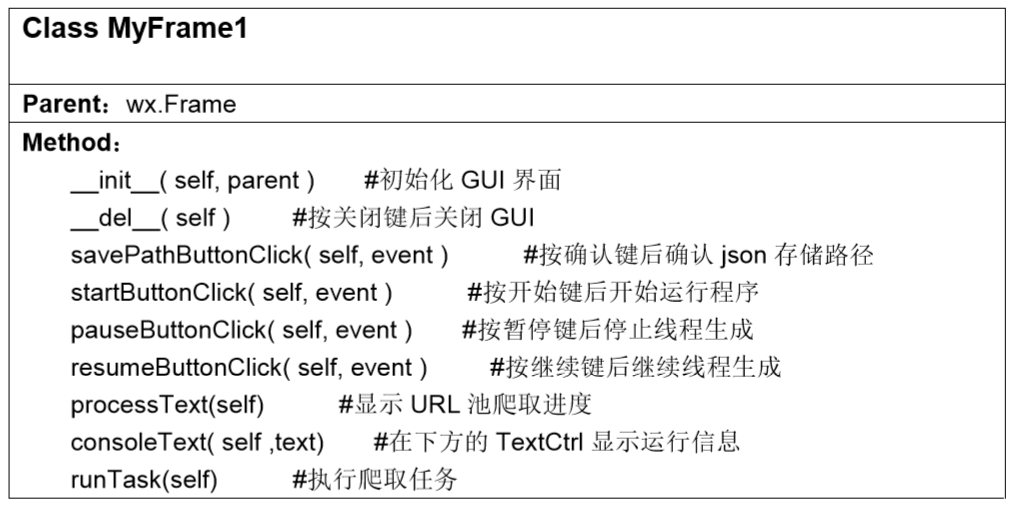
\includegraphics[width=10cm,height=5cm]{Myframe}
  \caption{Frame子类MyFrame1类设计}\label{Myframe}
\end{figure}
GUI界面如下图所示:
\begin{figure}[!htbp]
  \centering
  \begin{minipage}[t]{7.5cm}
    \centering
    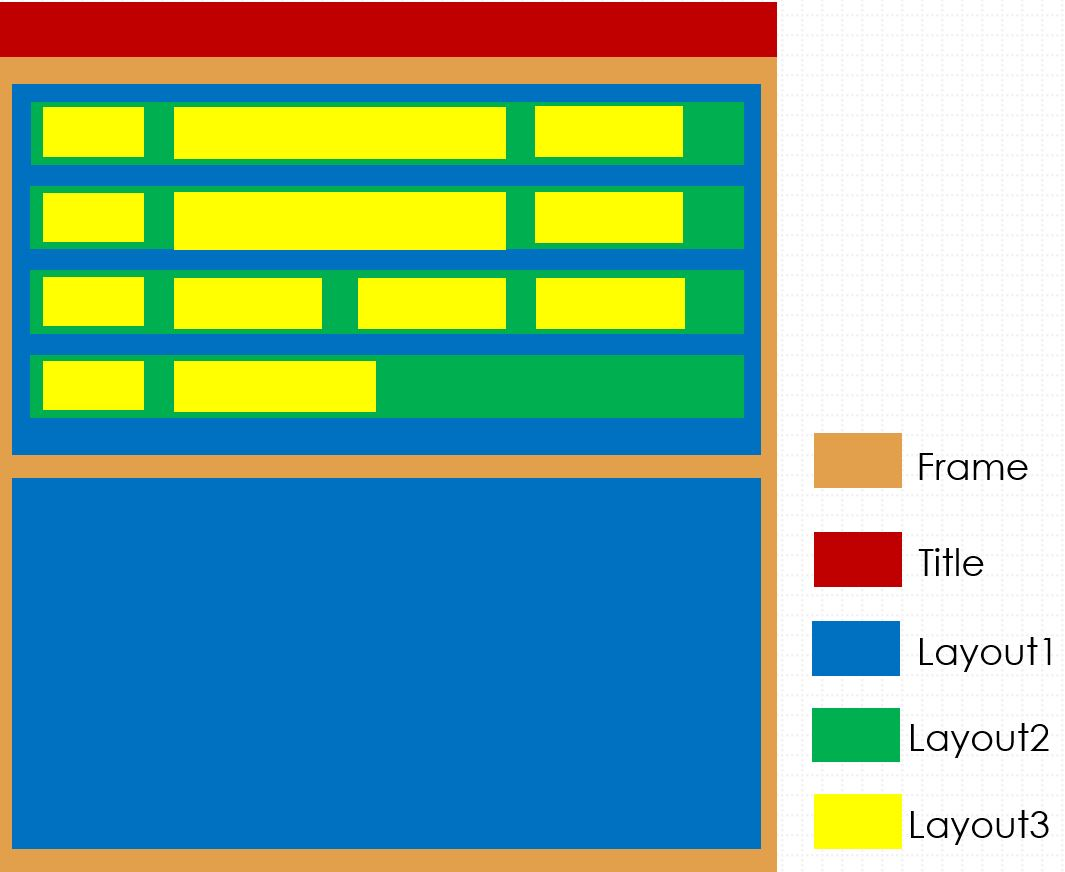
\includegraphics[width=7cm,height=6cm]{GUI设计}
    \centerline{\footnotesize{GUI设计}}
  \end{minipage}
  \begin{minipage}[t]{7.5cm}
    \centering
    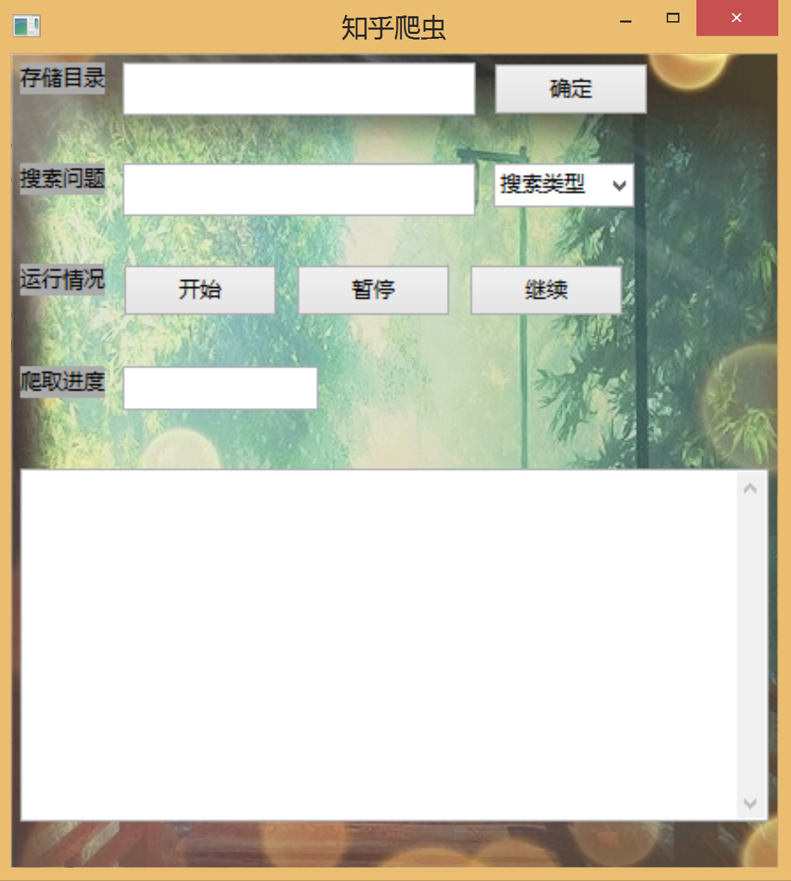
\includegraphics[width=6cm,height=6cm]{GUI界面}
    \centerline{\footnotesize{GUI界面}}
  \end{minipage}
  \caption{GUI}
\end{figure}

如上,左图是GUI的layout设计,右图是完成的GUI界面。该GUI界面的设计思路及方法是:在一个Frame上设置layout,在layout上可以叠加子layout或部件,layout可以选择水平排布和垂直排布,layout上的部件会按照设置自动排布。

在布局设计上,本工程使用了基于wxpython的平台wxFormBuilder进行辅助设计,通过该平台,可以很方便地实现部件的添加和事件的绑定,下图是该GUI设计的分级结构图:
\begin{figure}[!htbp]
  \centering
  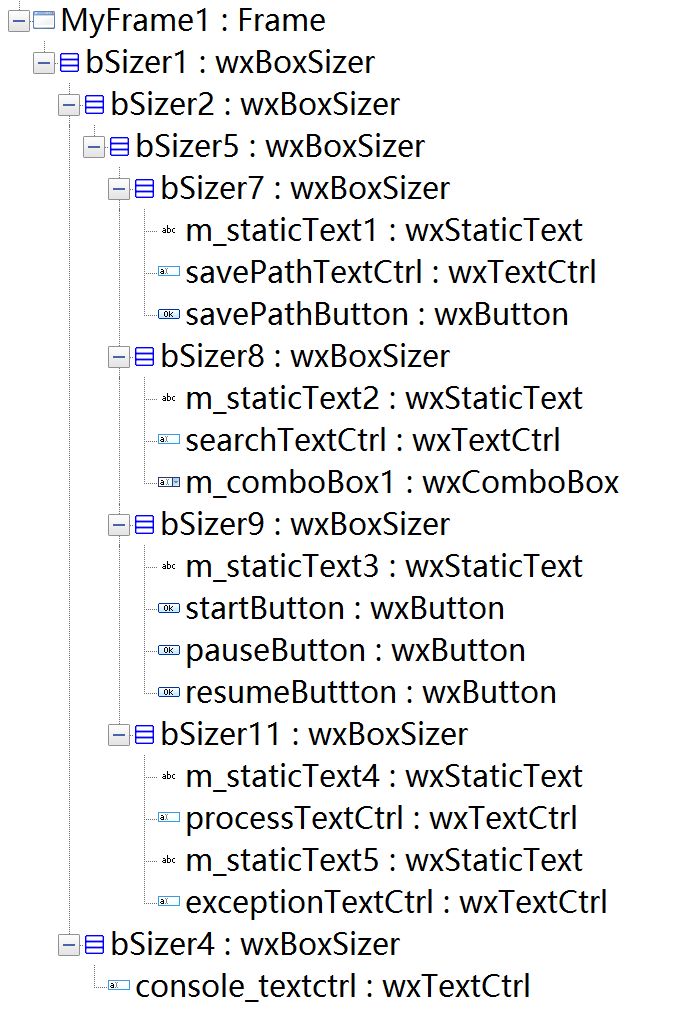
\includegraphics[width=6cm,height=7.5cm]{structure}
  \caption{分级结构图}\label{structure}
\end{figure}

在完成基础设计后,导出python代码,进行具体尺寸修改及bitmap背景设置,将爬虫控制程序绑定在GUI事件上,运行该类,即可实现爬虫程序的图形界面控制。

\subsubsection{多线程实现}
单线程爬取效率较低,对主机硬件资源的利用率较低,耗时也较长,因此,本工程使用python多线程库threading创建多线程任务提高爬取效率。

考虑到对于不同的搜索问题,本工程爬取的URL数不定,在创建新的爬取线程时我们直接创建匿名线程并启动。如下,调用crawl\_question函数并传入参数创建新线程:
\begin{lstlisting}[language=python]
threading.Thread(target=cq.crawl_question,args=(url,filename,)).start()
\end{lstlisting}
但若直接使用python的Thread类创建新线程,会面临一个问题:一个异常的线程会直接停止,并打印traceback异常,但使用无法知道是那个URL线程出了问题。对此,我们建立Thread类的子类,对父类的run方法进行覆写:
\begin{figure}[!htbp]
  \centering
  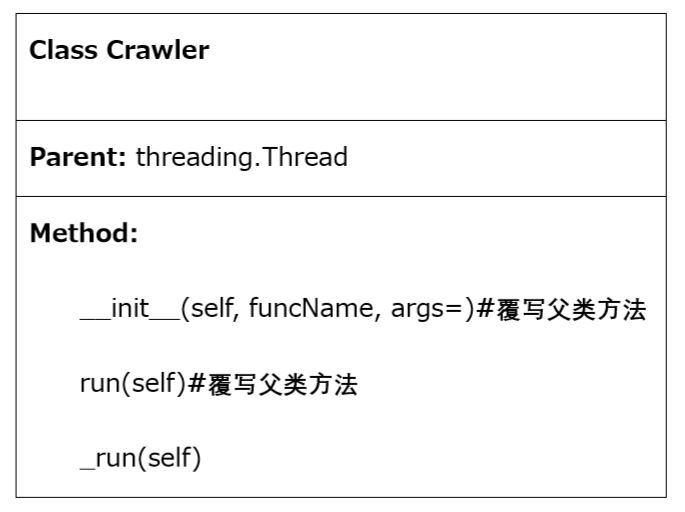
\includegraphics[width=7cm,height=4.5cm]{Thread}
  \caption{Thread子类Crawler类设计}\label{Thread}
\end{figure}
如上图,Crawler类覆写了父类的\_\_init\_\_方法和run方法,在run方法中调用\_run方法运行线程创建的目标函数,若运行期间出现异常,则抛出异常并打印异常信息及异常URL,代码如下:
\begin{lstlisting}[language=python]
import threading
import traceback
import sys
#Thread类的子类Crawler
class Crawler(threading.Thread):
    #class_lock = threading.Lock()

    def __init__(self,funcName=None,args=()):
        threading.Thread.__init__(self)
        self.args = args
        self.funcName = funcName
        self.exitcode = 0
        self.exception = None
        self.exc_traceback = ''
	
    #覆写run方法
    def run(self):
        try:
            self._run()
        except Exception as e:
            self.exitcode = 1
            self.exception = e
            self.exc_traceback = ''.join(traceback.format_exception(*sys.exc_info()))
            print("URL Crawler Exception: ", self.args[0])
            print(" self.exc_traceback")

    def _run(self):
        try:
            self.funcName(self.args[0],self.args[1])
        except Exception as e:
            raise e

\end{lstlisting}
在上面的代码中,创建Crawler类,父类为Thread类,覆写run方法,执行目标函数,若运行中出现问题,线程抛出异常,并打印出错误URL信息及traceback信息。

将Thread类改为Crawler类,匿名线程创建如下:
\begin{lstlisting}[language=python]
def crawl_web_into_json(url,filename):
   crawl_class.Crawler(funcName=cq.crawl_question,args=(url,filename,)).start()

\end{lstlisting}
在GUI中,当程序开始后,通过执行runTask方法调用crawl\_web\_into\_json创建爬取线程:
\begin{lstlisting}[]
def runTask(self):
		lock = threading.Lock()
		start = time.clock()
		while self.url_list:
				if (len(threading.enumerate())<11)&self.thread_flag :
						lock.acquire()
						url = self.url_list.pop(0)
						lock.release()
						zhihu_crawler.crawl_web_into_json(url, self.filename)
		elapsed = (time.clock() - start)

\end{lstlisting}

在程序运行中,当url\_list不为空,当程序总线程数小于11(最大多线程数为5)且程序未被暂停,url\_list弹出新url,并调用crawl\_web\_into\_json函数创建新线程。
在url\_list弹出新url过程中,为了防止资源竞争,对该步骤上锁,新线程创立后释放资源锁。
\begin{figure}[!htbp]
  \centering
  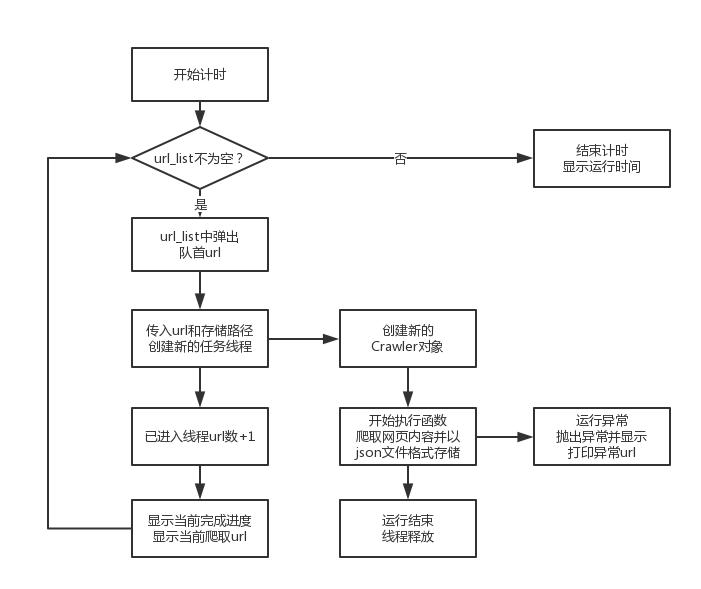
\includegraphics[width=9cm,height=8cm]{线程创建}
  \caption{线程创建流程图}\label{线程创建}
\end{figure}

经过测试,同一运行环境下,对于80条URL,单线程运行接近40分钟,而多线程运行可以把运行时间缩短到10分钟左右,大大提高了运行效率。
\newpage

\subsection{爬虫运行模块}
本模块主要实现了爬虫的基本运行,分为两个主要部分:
\vspace{-0.5cm}
\begin{itemize}
  \item 知乎登陆
  \item 建立问题URL库
  \begin{itemize}
    \item 针对具体问题(Question)搜索知乎的“综合”模块
    \item 针对具体话题(Topic)搜索知乎的“话题”模块
  \end{itemize}
\end{itemize}
\vspace{-0.3cm}
其中对问题(Question)的爬取采用PhantomJS库~\cite{bibtex2}来实现动态加载,对话题(Topic)的爬取采用模拟翻页来实现动态加载。其主要原理框图如下图所示:
\begin{figure}[!htbp]
  \centering
  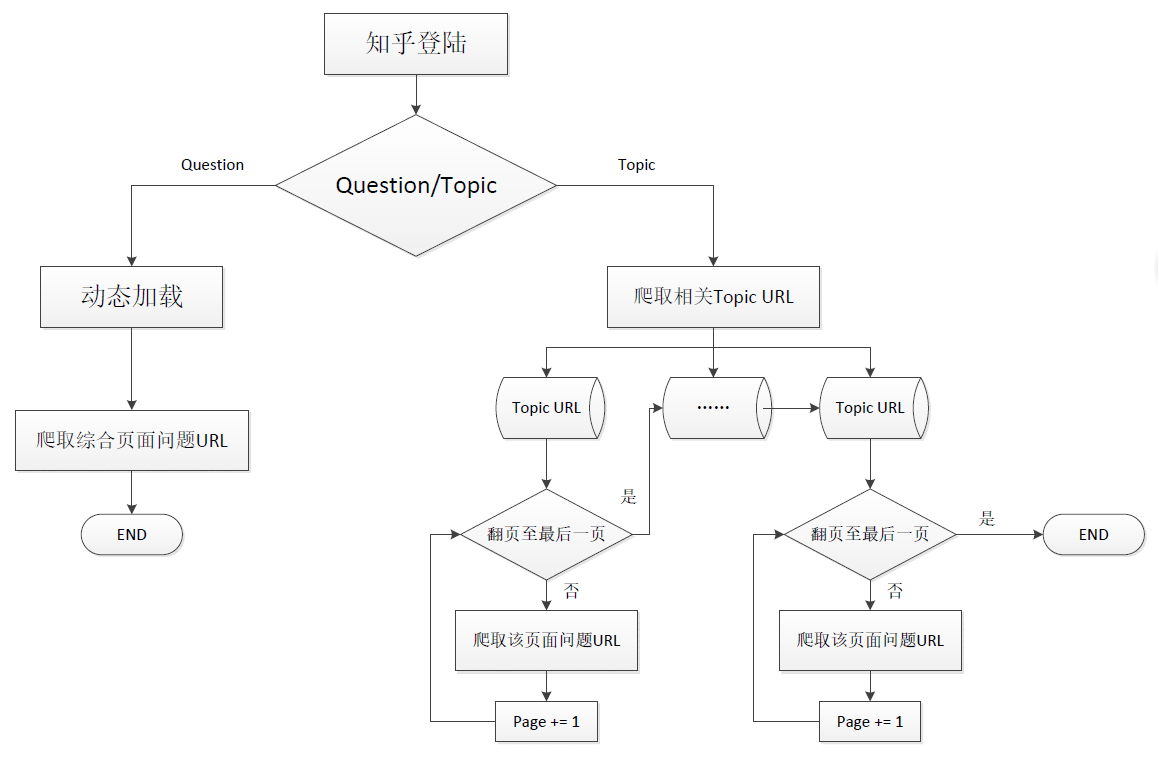
\includegraphics[width=15cm,height=10cm]{爬虫运行框图.png}
  \caption{爬虫运行框图}
\end{figure}
\subsubsection{知乎登陆}
知乎登陆是一个重要的环节,只有登录之后才可以捕捉到topic下面的所有页面信息。然而使用电脑浏览器登陆知乎需要点击倒立的文字,如果用程序模拟则十分不方便,速度也得不到保障;经尝试,我们可以使用手机的代理(User-Agent)来模拟登陆,此时request请求的头文件信息如下所示:
\begin{lstlisting}[language=python]
headers = {
    "Host": "www.zhihu.com",
    "Referer" : url,
    'X-Requested-With' : 'XMLHttpRequest',
    'User-Agent' : 'Mozilla/5.0 (Linux; Android 6.0; Nexus 5 Build/MRA58N)
                    AppleWebKit/537.36 (KHTML, like Gecko) Chrome/56.0.2924.87 Mobile Safari/537.36'
}
\end{lstlisting}

这时我们就可以用验证码来登陆,首先获取验证码的链接,然后使用request库访问链接抓取验证码图片并显示出来,等待用户输入。我们获取验证码的函数如下所示:
\begin{lstlisting}[language=python]
session = requests.session()
def get_captcha():
    t = str(int(time.time()*1000))
    captcha_url = url + 'captcha.gif?r=' + t + "&type=login"
    r = session.get(url=captcha_url, headers=headers)
    with open('captcha.gif', 'wb') as f:
        f.write(r.content)
        f.close()
    im = Image.open('captcha.gif')
    im.show()
    im.close()
    captcha = input("please input the captcha:")
    return captcha
\end{lstlisting}

登陆函数如下所示,可以使用手机号码或者是邮箱通过模拟post请求来登陆,如果返回状态码为200则说明登陆成功,我们会把登陆的信息打印出来以便测试。首次完成登陆后会保存用户的cookie,下次登陆可以直接加载cookie而不需要再次输入账号和验证码。
\begin{lstlisting}[language=python]
def login(secret, account):
    if re.match(r"^1\d{10}$", account):
        # login with phone number
        post_url = 'https://www.zhihu.com/login/phone_num'
        postdata = {
            'phone_num': account,
            'password' : secret
        }
    else:
        # login with email
        post_url = url + 'login/email'
        postdata = {
            'email' : account,
            'password': secret
        }
    # with captcha
    postdata["captcha"] = get_captcha()
    login_page = session.post(url=post_url, headers=headers, data=postdata)
    print('the status code returned by server:', login_page.status_code)
    if login_page.status_code != 200:
        print('login error!')
    else:
        print(login_page.json())
        while login_page.json()['r'] == 1:
            postdata["captcha"] = get_captcha()
            login_page = session.post(url=post_url, headers=headers, data=postdata)
            print('the status code returned by server:', login_page.status_code)
            print(login_page.json())

    session.cookies.save()
\end{lstlisting}
登陆函数测试结果如下:
\vspace{1.3cm}
\begin{lstlisting}[language=XML]
C:\Users\dell-pc\Anaconda3\python.exe C:/Users/dell-pc/Desktop/zhihu_crawler_py3/login.py
Cookie cannot be load!
your name:  None
please input your account:******
please input your secret:******
please input the captcha:f8dk
the status code returned by server: 200
{'r': 0, 'msg': '登录成功'}
your name:  <span class="name">游浩然</span>
\end{lstlisting}

\subsubsection{网页下载\&解析}
网页下载函数即为下代码所示,使用requests库来抓取指定URL的内容:
\begin{lstlisting}[language=python]
def getHTMLText(url):
    try:
        r = requests.get(url, headers=headers)
        # r.status_code    200
        # r.encoding    'utf-8'
        return r.content
    except:
        return "Error"
\end{lstlisting}

网页解析则依赖于BeautifulSoup库,比如下代码中demo即为爬取的网页内容,通过BeautifulSoup解析过后以网页标签来爬取相应问题的URL。
\begin{lstlisting}[language=python]
demo = demo_temp.pop()
soup = BeautifulSoup(demo, 'html.parser')
for meta in soup.find_all('meta', attrs={'itemprop': 'url'}):
    url_temp = meta.get('content')
    url_list.append(url_temp)
\end{lstlisting}
\subsubsection{URL爬取\&管理}
\begin{itemize}
  \item 对知乎“综合”模块进行爬取 \\
  采用PhantomJS来模拟对页面的下拉操作来实现动态加载,之后获取该URL的HTML页面,使用BeautifulSoup来解析,利用网页中的<meta>标签的content属性来抓取页面上的所有问题链接,补充入地址池。
  \begin{lstlisting}[language=python]
  def get_content(url, url_list):
    driver = webdriver.PhantomJS(executable_path=r"E:/phantomjs/bin/phantomjs.exe")
    driver.implicitly_wait(10)
    driver.maximize_window()
    driver.get(url)

    demo_temp = []
    time.sleep(1)
    while True:
        if len(demo_temp) > 10:
            demo_temp = demo_temp[-10:]
            if demo_temp[0] == demo_temp[9]:
                break
        driver.execute_script('window.scrollTo(0,document.body.scrollHeight)')
        time.sleep(1)
        demo_temp.append(driver.page_source)

    demo = demo_temp.pop()
    soup = BeautifulSoup(demo, 'html.parser')
    for meta in soup.find_all('meta', attrs={'itemprop': 'url'}):
        url_temp = meta.get('content')
        url_list.append(url_temp)
    return url_list

    if DType == 'question':
    # get a question url
    content = {'' : content}
    url = "https://www.zhihu.com/search?type=content&q" + urllib.parse.urlencode(content)
    # search url in this page
    url_list = URL.get_content(url, [])
  \end{lstlisting}
  \begin{figure}[!htbp]
    \centering
    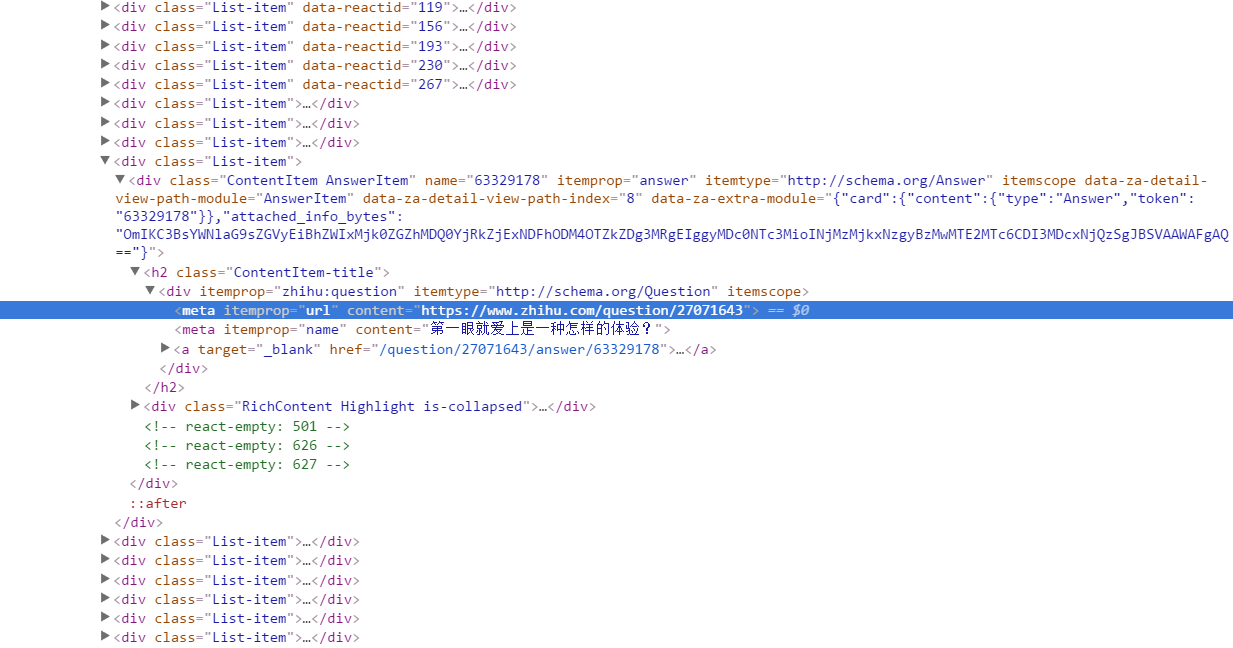
\includegraphics[width=15cm,height=8.5cm]{meta}
    \caption{HTML文件中的<meta>标签}\label{meta}
  \end{figure}
  \item 对知乎“话题”模块进行爬取 \\
  首先由种子URL开始,爬取相关topic的URL,如下函数:
  \begin{lstlisting}[language=python]
  def get_topic_id(url, url_list):
    demo = getHTMLText(url)
    soup = BeautifulSoup(demo, "html.parser")
    for link in soup.find_all('a'):
        url_temp = link.get('href')
        if not url_temp:
            pass
        elif '/topic' in url_temp and not 'http' in url_temp:
            topic_id = url_temp[7:15]
            url_list.append('https://www.zhihu.com/topic/' + topic_id)
    return url_list
  \end{lstlisting}
  针对前述的每一个URL,爬取该topic下的所有问题,只需要解析出其问题的总页数,通过page+=1的操作模拟翻页过程,爬取该topic下面的所有问题的URL补充进地址池。\\
  \begin{figure}[!htbp]
    \centering
    
\includegraphics[width=10cm,height=1cm]{page}
    \caption{Topic下所有问题页数}\label{page}
  \end{figure}

  \begin{lstlisting}[language=python]
  def get_question_id(url, url_list):
    page_url = url + '/questions?page=1'
    demo = getHTMLText(page_url)
    soup = BeautifulSoup(demo, "html.parser")
    # get total page
    num_page = 1
    for link in soup.find_all('a'):
        url_temp = link.get('href')
        if '?page=' in url_temp:
            num_page = max(num_page, int(url_temp[6:len(url_temp)]))
    print('the number of page in topic ' + url[28:len(url)] + ' is : ' + str(num_page))
    # get all questions under topic
    for page in range(1, num_page+1):
        page_url = url + '/questions?page=' + str(page)
        demo = getHTMLText(page_url)
        soup = BeautifulSoup(demo, "html.parser")
        for link in soup.find_all('a'):
            url_temp = link.get('href')
            if '/question' in url_temp and not 'http' in url_temp:
                question_id = url_temp[10:19]
                url_list.append('https://www.zhihu.com/question/' + question_id)
    return url_list
  \end{lstlisting}
  对知乎“话题”模块所有问题URL进行爬取并管理的代码如下所示:
  \begin{lstlisting}[language=python]
    if DType == 'topic':
    # get a topic url
    url = "https://www.zhihu.com/search?type=topic&q=" + content

    # search url in this page
    url_temp = URL.get_topic_id(url, [])
    if len(url_temp) > 0:
        url_list = url_list + url_temp

    # duplicate removal
    url_list = list(set(url_list))

    # search url based on BFS
    if len(url_list) > 0:
        url = url_list[0]
    while '/topic' in url and len(url_list) > 0:
        url = url_list.pop(0)
        url_temp = URL.get_question_id(url, [])
        if len(url_temp) > 0:
            url_list = url_list + url_temp

    # duplicate removal
    url_list = list(set(url_list))
    return url_list
  \end{lstlisting}
\end{itemize}
\newpage

\subsection{数据输出模块}
\subsubsection{Question页面动态加载}
首先,由于知乎问题页面采用了动态加载技术,直接通过url获取的网页内容只有一小部分,其次,虽然通过浏览器请求可以得到回答的json数据,但由于问题的完整描述需要执行点击操作,故最终考虑使用selenium模拟浏览器操作,在实际爬取中,我们采用了PhantomJS(基于webkit的没有界面的浏览器),相较于Chrome和FireFox有更快的速度。

实现难点:由于selenium是通过模拟浏览器来获取网页内容,所以存在一个加载以及渲染过程,也就是说在执行每步操作后,需要让程序等待一段时间。另外在回答加载上,需要不断将鼠标下滑到页面底部,由于存在加载的时间,故要控制该行为的频率,以免造成过多的无效操作。

代码实现:

\begin{lstlisting}[language=python]
# 点击操作
try:
    click_btn = driver.find_element_by_xpath('//button[@class="Button QuestionRichText-more Button--plain"]')
    ActionChains(driver).click(click_btn).perform()
    time.sleep(0.5)
    html_text = driver.page_source
except:
    html_text = driver.page_source
# 下滑操作
while(True):
    driver.execute_script('window.scrollTo(0,document.body.scrollHeight)')
    time.sleep(0.8)
    if(html_text == driver.page_source):
        break
    html_text = driver.page_source

\end{lstlisting}

\subsubsection{Question网页解析}
网页解析要求从HTML中提取所需的信息,我们选取的工具是beautifulsoup4,相较于采用xpath,css以及正则表达式,更加方便简洁。

实现难点:需要通过浏览器检查元素来确定元素的位置,以及如何利用条件来提取该位置的元素。

代码实现:
\begin{lstlisting}[language=python]
# 获取问题标题
question_title = soup.select_one('h1[class="QuestionHeader-title"]').get_text()
question_dict['question_title'] = question_title

# 获取回答
nodes = soup.find_all('div', class_="List-item")
\end{lstlisting}

\subsubsection{Question数据存储}
由于json能较好地的反映数据的从属关系,并且更加易读,所以我们决定将爬取的数据保存成json格式~\cite{bibtex3}。

实现难点:Python对于中文字符的支持不够好,在保存时需要转换成unicode编码。

\begin{itemize}
  \item 代码实现:
  \begin{lstlisting}[language=python]
    with open(file_name, 'wb') as json_file:
        for info in info_list:
            json_file.write(json.dumps(info,ensure_ascii=False).encode('utf-8'))
            json_file.write('\n'.encode('utf-8'))
  \end{lstlisting}
\end{itemize}

效果展示:
\begin{itemize}
  \item 问题信息
  \begin{lstlisting}[language=json]
  {
    "question_followers": "15,436",
    "question_title": "如何在四小时内学会用 Ai 做 UI?",
    "answer_number": "86 个回答",
    "question_text": "整个问题的初衷在于看到了@黎敏 的回答,产品经理新人是否有必要学习Photoshop? 我这个问题主要在于希望一些新人能速度的进入AI操作,而不必花时间去找教程,需要这个问题回答的人不少。再次谢谢 @黎敏。",
    "question_commet": "15 条评论",
    "brower_number": "989,872",
    "question_id": "21378038"
  }
  \end{lstlisting}
  \item 回答信息
  \begin{lstlisting}[language=json]
  {
    "answer_votes": "0",
    "answer_author": "mac mico",
    "answer_text": "工欲善其事必先利其器,效率一定是首要的。UI设计之效率为王 - 设计与开发之效率 - 知乎专栏",
    "answer_id": 61575458,
    "answer_comment": "添加评论"
  }
  \end{lstlisting}
\end{itemize}
\newpage

\subsection{爬虫测试效果}
\begin{itemize}
  \item 爬虫正常运行!
\end{itemize}
\begin{figure}[!htbp]
  \centering
  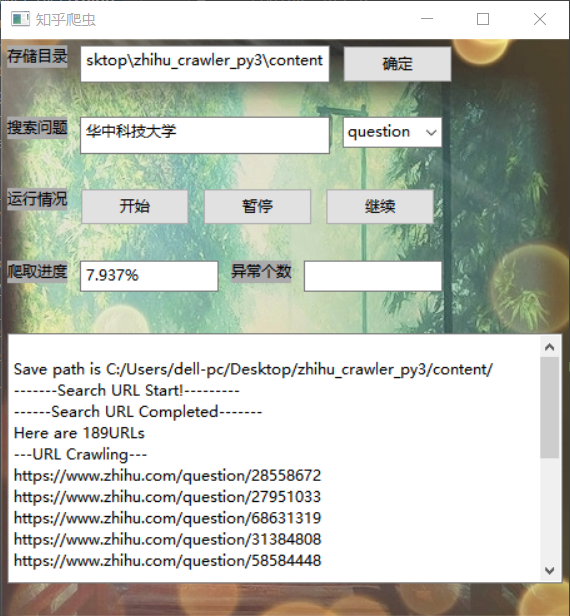
\includegraphics[width=10cm,height=10cm]{爬取}
  \caption{爬取程序运行效果}
\end{figure}

\section{项目分工}

\begin{table}[!htbp]
  \centering
  \renewcommand\arraystretch{1.5}
 	\resizebox{\textwidth}{!}{
    \begin{tabular}{|c|c|c|c|}
 		\hline
 		\qquad ~~姓名~~~~~  & \qquad ~~负责模块~~~~~ & \qquad ~~主要任务~~~~  \\
 		\hline
        \qquad ~~黎张帆~~~~  & \qquad ~~爬虫控制器~~~ & \qquad ~~启动、停止、监视爬虫的运行情况;实现多线程爬取。GUI设计~~~ \\
        \hline
        \qquad ~~游浩然~~~~  & \qquad ~~爬虫运行模块~~~ & \qquad ~~知乎登陆;URL管理器、网页下载器、网页解析器;动态加载~~~ \\
        \hline
        \qquad ~~郭金城~~~~  & \qquad ~~数据输出模块~~~ & \qquad ~~通过网页标签抓取问题URL下的相关信息;动态加载~~~ \\
        \hline
 	\end{tabular}
    }
 \end{table}
\newpage

\section{设计总结}

通过这次软件课程设计,我更好地理解了爬虫运行的原理,包括模拟登陆、网页下载、网页解析以及动态加载,更好地了解了Python中的requests、BeautifulSoup、re、http等等爬虫常用的库。

在实验过程中也遇到了许多问题,比如知乎登陆过程中如果使用PC端的User-Agent则会有点击倒立的验证码的操作,影响实验效率,我为此专门尝试其他浏览器代理登陆,发现手机端登陆只需要输入验证码即可,节约了时间;还比如在处理搜索“question”时综合页面动态加载的过程中,开始的时候积极尝试各种方法,比如通过浏览器抓包获得页面数total和当前页面page的内容以及下一页面的url链接,这样就可以更快地去抓取所有页面,但是由于知乎的反爬机制,使用requests库不能获取到服务器内部信息,最后选择了使用selenium来模拟浏览器下滑的过程实现动态加载;但在处理搜索“topic”时爬取全部问题时,网页是存在具体的页面的,这时只需要翻页即可!实现动态加载的过程也教会了我“分而治之”的思想,对于具体的问题要有相对应的解决方法,不能拘泥于已有的了解一概而论。

亲自动手实践让我巩固了python的基础应用、掌握了爬虫的工作模式以及领会到“分而治之”的灵活思想,受益匪浅!



\newpage

\bibliographystyle{unsrt}
%\bibliographystyle{plain}%
\bibliography{bibfile}

\end{document} 